% !TEX encoding = UTF-8 Unicode
\documentclass[10pt]{book}
\usepackage[utf8]{inputenc}
\usepackage[ngerman]{babel}

\usepackage{geometry}
\geometry{a5paper}
\usepackage[parfill]{parskip}
\usepackage{graphicx}
\usepackage{amssymb}
\usepackage{multirow}
\usepackage[lastexercise]{exercise}
\usepackage{tikz}
\usetikzlibrary{positioning,fit}

\title{Mikrocomputer}
\author{Katrin Spahn}
\date{\today}

\begin{document}
\maketitle

\tableofcontents

\chapter{Schneller Einstieg}

Das erste Kapitel soll dir einen genauen Einblick
in die Bedienung, die Funktionsweise
und in den Aufbau des Mikrocomputers geben.

\section{Checkliste}
Bevor du den Mikrocomputer anschließen und einschalten
kannst, solltest du überprüfen, ob du auch alle Dinge
hast, die du zum Arbeiten mit dem Mikrocomputer brauchst.

%Checkliste
\begin{itemize}
\item Mikrocomputer
\item Bildschirm mit VGA-Anschluss
\item Netzteil
\item PS/2-Tastatur 

\end{itemize}
Du kannst auch eine USB-Tastatur
und dazu einen Adapter für die
PS/2 Schnittstelle nehmen.
Allerdings unterstützt nicht jede USB-Tastatur
einen Adapter für die PS/2-Schnittstelle.
Benutze also am besten eine USB-Tastatur,
wo der Adapter gleich mit dabei ist.


\section{Anschließen und Einschalten}

Die kleine schwarze Buchse links
ist der Anschluss für das Netzteil.
Den runden Stecker des Netzteiles kannst
ohne weiteres Bedenken in die Buchse schieben.
In die lilane Buchse kommt der PS/2-Stecker,
schau dir den Stecker genau an und stecke ihn
ohne Gewalt richtig herum rein.
Zur Orientierung schaue
Abildung \ref{fig:ps2connector} an.
Den schmalen Bildschirmstecker nun noch
in die Buchse rechts stecken
und nun kann der Anschaltkopf
auf der linken Seite betätigt werden.
Auf dem Bilschirm müsste der
Maschinencode-Monitor wie in
Abblidung \ref{fig:monitorscreenshot} erscheinen.

Den Maschiencode-Monitor verstehen

Wenn du bereits den Mikrocomputer angeschaltet hast solltest du
den Maschinencode-Monitor sehen. Unter Abildung \ref{fig:monitorscreenshot}
kannst du den
Maschinencode-Monitor betrachten. Doch jetzt wollen wir den Maschinen-code vorallem verstehnen, wir fangen dabei ganz oben an. Die oberste zeile ist das Menü.
Du kannst verschiedene Befehle wählen, hinter den Befehlen steht was diese tun.
Gehnen wir nun eine zeile weiter nach unten, ganz links steht in einen extra Käschen die jeweilige Seitenzahl. Mit PgUp und PgDn kannst du die seiten wechseln.
Neben der Seitenzahl steht die spaltennummern,  darunter siehst du auch die Spalten, die im Moment noch Nullen sein dürften. Links unter der Seitenzahl sind die Zeilennummern. Die Seitenzahl, die Zeilennumern, die Spaltennummern dienen zum Ablesen der Speicheradresse. 
Gehe mal zum Anfang der Zeile mit den Nullen und gebe F1 ein
\begin{figure}
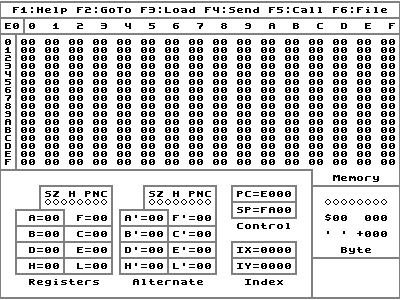
\includegraphics[width=\textwidth]{monitor.png}
\caption{Der Maschinencode-Monitor}
\label{fig:monitorscreenshot}
\end{figure}

\section{Der Speicher des Computers}

Der Computer arbeitet mit Bits.
Ein Bit hat immer einen von zwei möglichen Zuständen.
Es ist entweder ``an'' oder ``aus''.
Man schreibt dafür auch ``1 oder ``0''.
Andere Bezeichnungen wären ``Ja'' oder ``Nein''
sowie ``High'' oder ``Low''.
Wie man es nennt, ist nicht wichtig.
Es geht nur darum, dass es außer diesen beiden Möglichkeiten
keine weiteren gibt.
Das ist ein 8 Bit Rechner.
Das heißt das immer 8 Bit als Einheit verarbeitet werden.
Diese Einheit nennt man Byte.
Es gibt 256 Möglichkeiten wie ein Byte aussehnen kann.
Doch einzelne Bits aufzuschreiben wird unübersichtlich
deswegen verwendet man die Hexadezimalschreibweise.
Dazu teilt man das Byte in Zwei Hälfen zu je 4 Bit.
Ein solches Halbbyte nennt man Nibble. 
Für ein Nibble gibt es nur noch 16 verschiedene
Möglichkeiten wie es aussehen kann.

In der Hexadezimalschreibweise gibt es 16 Ziffern.
Zu ihnen gehören die Ziffern 0-9
und die Bustaben A-F müssen hier
auch als Ziffern herhalten,
sodass wir ingesamt 16 Ziffern haben.

\section{Hello, world!}
Nun gib das Programm aus
Tabelle \ref{tab:helloworldcode} ein.
Wenn du es fertig abgetippt hast,
sollte ``Hello, world!'' auf dem Bildschirm erscheinen.
Fange oben links in der ersten Zeile an
und benutze einfach die Pfeiltasten zum Weiterspringen.
Zum Ausführen des Programmes gehe an den Anfang der ersten Zeile und drücke F5.
Jetzt sollte auf dunkelgrünen Hintergrund in weißen Buchstaben
Hello World! stehen. Um das Programm wieder zu Beenden drücke die ESC-Taste.
\begin{table}
\centering
\setlength{\tabcolsep}{3pt}
\texttt{
\begin{tabular}{ r | rrrrrrrrrrrrrrrr }
E0 &  0& 1& 2& 3& 4& 5& 6& 7& 8& 9& A& B& C& D& E& F \\
\hline
 0 & CD&11&07&21&16&E0&FD&21&41&00&CD&32&08&CD&E8&04 \\
 1 & 3E&1B&B9&20&F8&C9&48&65&6C&6C&6F&2C&20&77&6F&72 \\
 2 & 6C&64&21&00 \\
\end{tabular}
}
\caption{``Hello, world!'' in Maschinencode}
\label{tab:helloworldcode}
\end{table}

Doch wenn es nun geklappt hat,
willst du bestimmt wissen,
wie dieses Programm funktioniert.


Jedes Byte hat in der Hexadezimalschreibweise
zwei dieser Ziffern.
Manche Kominationen sind widerum
bestimmten Zeichen zugeordnet.
Um das näher zu Verstehnen, löse folgende Aufgaben.
Die Lösungen findest du am Ende des Kapitels
auf Seite \pageref{sec:solutions1}.

\begin{Exercise}[label=ex:asciidecode]
In der Tabelle 1.2 sind
in der Hexadezimalschreibweise Bytes aufgeführt,
die wiederum bestimmten Zeichen zugeordnet sind.
Auch das Hello-World-Programm besteht aus
in der Hexadezimalschreibweise geschriebenen Bytes.
Mansche Bytes im Programm sind bestimmten Zeichen zugeordnet.
Finde mit Hilfe der Tabelle \ref{tab:ascii} heraus,
welche Bytes bestimmte Symbole haben
und schreibe diese auf.
Findest du heraus wo der Text ``Hello, World!''
sich im Programm verbirgt?
\end{Exercise}

\begin{table}
\centering
\newcommand{\bs}{\textbackslash}
\begin{tabular}{ | rc | rc | rc | rc | rc | rc |}
\hline
\texttt{20} & ~    & \texttt{30} & 0    & \texttt{40} & @ &
\texttt{50} & P    & \texttt{60} & \`{} & \texttt{70} & p \\
\texttt{21} & !    & \texttt{31} & 1    & \texttt{41} & A &
\texttt{51} & Q    & \texttt{61} & a    & \texttt{71} & q \\
\texttt{22} & "    & \texttt{32} & 2    & \texttt{42} & B &
\texttt{52} & R    & \texttt{62} & b    & \texttt{72} & r \\
\texttt{23} & \#   & \texttt{33} & 3    & \texttt{43} & C &
\texttt{53} & S    & \texttt{63} & c    & \texttt{73} & s \\
\texttt{24} & \$   & \texttt{34} & 4    & \texttt{44} & D &
\texttt{54} & T    & \texttt{64} & d    & \texttt{74} & t \\
\texttt{25} & \%   & \texttt{35} & 5    & \texttt{45} & E &
\texttt{55} & U    & \texttt{65} & e    & \texttt{75} & u \\
\texttt{26} & \&   & \texttt{36} & 6    & \texttt{46} & F &
\texttt{56} & V    & \texttt{66} & f    & \texttt{76} & v \\
\texttt{27} & '    & \texttt{37} & 7    & \texttt{47} & G &
\texttt{57} & W    & \texttt{67} & g    & \texttt{77} & w \\
\texttt{28} & (    & \texttt{38} & 8    & \texttt{48} & H &
\texttt{58} & X    & \texttt{68} & h    & \texttt{78} & x \\
\texttt{29} & )    & \texttt{39} & 9    & \texttt{49} & I &
\texttt{59} & Y    & \texttt{69} & i    & \texttt{79} & y \\
\texttt{2A} & *    & \texttt{3A} & :    & \texttt{4A} & J &
\texttt{5A} & Z    & \texttt{6A} & j    & \texttt{7A} & z \\
\texttt{2B} & +    & \texttt{3B} & ;    & \texttt{4B} & K &
\texttt{5B} & [    & \texttt{6B} & k    & \texttt{7B} & \{ \\
\texttt{2C} & ,    & \texttt{3C} & $<$  & \texttt{4C} & L &
\texttt{5C} & \bs  & \texttt{6C} & l    & \texttt{7C} & $|$ \\
\texttt{2D} & -    & \texttt{3D} & =    & \texttt{4D} & M &
\texttt{5D} & ]    & \texttt{6D} & m    & \texttt{7D} & \} \\
\texttt{2E} & .    & \texttt{3E} & $>$  & \texttt{4E} & N &
\texttt{5E} & \^{} & \texttt{6E} & n    & \texttt{7E} & \textasciitilde \\
\texttt{2F} & /    & \texttt{3F} & ?    & \texttt{4F} & O &
\texttt{5F} & \_{} & \texttt{6F} & o    & \texttt{7F} & $\blacksquare$ \\
\hline
\end{tabular}
\caption{ASCII-Zeichensatz}
\label{tab:ascii}
\end{table}

\begin{Exercise}[label=ex:asciiencode]
Der Text aus dem Hello-Wolrd-Programm
kann natürlich auch ge\-än\-dert werden.
Und zwar indem du die Bytes,
die du in Übung \ref{ex:asciidecode} gefunden hast,
durch Bytes ersetzt, die andere Symbole haben.
Denke dir also deinen eigenen Text aus.
Dieser Text kann alles Mögliche sein,
vieleicht dein Lieblingsessen oder dein Hobby,
der Name deines Haustieres
oder irgendetwas anders was dir gerade einfällt.
\end{Exercise}

Nun weist du was die Bytes nach C9 zu bedeuten haben,
denn da befindet sich ja unser Text der auf denn Bildschirm ausgegeben wird.
Aber was bezweken die Bytes davor? Die Bytes davor haben natürlich auch ihre Aufgabe.

1. CD 11 07		Löschen des Bildschirms

2. 21 16 E0		Text von Speicheradresse E016

3. FD 21 41 00		an Grafikadresse 0041

4. CD 32 08		ausgeben

5. CD E8 04		welche Taste wurde gedrückt?

6. 3E 1B B9		War das die ESC-Taste?

7. 20 F8		wenn nicht, dann springe zurück (zu 5.)

8. C9			Programmende


Diese Bytes die du in Hexadezimalschreibweise
eingegenben hast, das ist direkt der Maschienencode.
In dieser Dokumentation wird Assembler verwendet.
In Assembler gibt es Abkürzungen
anstelle des Maschiencodes,
die dannn in Maschiencode übersetzt werden.
Doch diese Buchstaben Abkürzungen in Assembler
sind zwar Befehle aber lösen keine komplexen Probleme.
Dies bedeutet um etwas Bestimmtes zu erreichen,
muss man verstehen wie die Komponenten
des Rechners miteinander zusammen arbeiten.

\section{Bitte Überschrift einsetzen}

Ziel: Hintergrundfarbe ändern (eigenes Programm)

\begin{figure}
\centering
\begin{tikzpicture}[align=center,
	conn/.style={line width=2pt,stealth-stealth},
	box/.style={rectangle,draw,text width=2cm,minimum size=1.5cm}]
\node[box](cpu){eZ80 CPU};
\node[box](bus)[below=of cpu]{Bus \\ Controller};
\node[box](ram)[below=of bus]{RAM};
\node[box](rom)[below right=of bus]{Flash \\ Memory};
\node[box](spi)[below left=of bus]{Serial \\ Peripheral \\ Interface};
\node[rectangle,draw,fit=(cpu)(bus)(ram)(rom)(spi),label={eZ80 Mikrocontroller}](mcu){};
\node[box](gpu)[below=of spi]{Grafikchip};
\node(mon)[right=of gpu]{Monitor};
\draw[conn](cpu) to (bus);
\draw[conn](bus) to [out=-90,in=90] (ram);
\draw[conn](bus) to [out=-90,in=90] (rom);
\draw[conn](bus) to [out=-90,in=90] (spi);
\draw[conn](spi) to (gpu);
\draw[->](gpu) to (mon);
\end{tikzpicture}
\caption{Komponenten des Mikrocomputers (Ausschnitt)}
\label{fig:componentssimple}
\end{figure}

\clearpage\section*{Lösungen zu den Aufgaben im Text}
\label{sec:solutions1}
\begin{Answer}[ref=ex:asciidecode]
Wenn du die Aufgabe richtig gelöst hast,
solltest du tatsächlich in dem Programm
den Text ``Hello World!'' gefunden haben.
Dieser ist ganz am Ende des Programmes versteckt
und zwar in den folgenden Bytes:
\begin{center}
\setlength{\tabcolsep}{3pt}
\begin{tabular}{ c | ccccccccccccc | c }
\hline
\multirow{2}{*}{\dots} &
\texttt{48} & \texttt{65} &\texttt{6C} &
\texttt{6C} & \texttt{6F} &\texttt{2C} &
\texttt{20} & \texttt{77} &\texttt{6F} &
\texttt{72} & \texttt{6C} &\texttt{64} &
\texttt{21} &
\multirow{2}{*}{\dots} \\
&H&e&l&l&o&,& &W&o&r&l&d&!& \\
\hline
\end{tabular}
\end{center}
\end{Answer}

\begin{Answer}[ref=ex:asciiencode]
In der Beispiellösung wurde der Text
``Hello, World!'' durch den Text
``APFELKUCHEN SCHMECKT GUT!'' ersetzt.
Hierbei wurden nur Bytes verwendet,
die als Symbole Großbuchstaben haben.
Du kannst aber natürlich auch
normal Groß- und Kleinbuchstaben verwenden.
\begin{center}
\setlength{\tabcolsep}{3pt}
\texttt{
\begin{tabular}{ r | rrrrrrrrrrrrrrrr }
E0 &  0& 1& 2& 3& 4& 5& 6& 7& 8& 9& A& B& C& D& E& F \\
\hline
 0 & CD&11&07&21&16&E0&FD&21&41&00&CD&32&08&CD&E8&04 \\
 1 & 3E&1B&B9&20&F8&C9&41&50&46&45&4C&4B&55&43&48&45 \\
 2 & 4E&20&53&43&48&4D&45&43&4B&54&20&47&55&54&21&00 \\
\end{tabular}
}
\end{center}
\end{Answer}

\chapter{Hier Titel einfügen}

\end{document}